\documentclass[11pt]{article}
\usepackage[margin=1in]{geometry}
\usepackage{amsmath,amssymb,amsthm}
\usepackage{booktabs,multirow,graphicx,xcolor}
\usepackage[numbers,sort&compress]{natbib}
\usepackage{lmodern}
\usepackage[T1]{fontenc}
\usepackage{microtype}
\usepackage{hyperref}
\usepackage{draftwatermark}
\SetWatermarkText{PRIVATE DRAFT}
\SetWatermarkScale{0.6}
\SetWatermarkLightness{0.93}
\hypersetup{colorlinks=true,linkcolor=blue!50!black,citecolor=blue!50!black,urlcolor=blue!50!black}
\graphicspath{{../figures/}}
\newcommand{\pending}[1]{\textcolor{orange!70!black}{\emph{pending: #1}}}
\newcommand{\E}{\mathbb{E}}

\title{A Race of Delayed Clocks:\\ Exact, Compact Marked Point Processes\\ and the Recording-Resolution Pitfall}
\author{Tero Keski-Valkama \and Karoliina Salminen\\ \small Sleeping Machines}
\date{Private draft, 7 October 2026 --- not for distribution before the disclosure decision}

\begin{document}
\maketitle

\begin{abstract}
We model the next event of a marked temporal point process as the winner of a race between independent clocks started at the previous event: exponential clocks, delayed clocks that fire only with a learned probability, flat delay windows with learned soft edges, and a state clock whose hazard follows a persistent memory that keeps evolving through the silent interval. Each clock carries its own mark distribution, so the predicted event type depends on elapsed time through which clock is likely to win. Apart from the state clock, every term of the likelihood is closed-form: no Monte Carlo compensator is needed, and every losing clock receives exact credit through its survival factor. On EasyTPP with its official splits and the per-event log-likelihood protocol of the current state of the art, the model exceeds the best published result on Taobao ($1.399 \pm 0.003$ vs.\ $1.318$ nats/event), Taxi ($0.525 \pm 0.001$ vs.\ $0.522$, using $1/12$ of the leading model's parameters and per-event compute; a five-model mixture reaches $0.536$ at $0.41\times$ its compute) and StackOverflow ($-2.144 \pm 0.004$ vs.\ $-2.163$), five seeds each. We further show that continuous-time models can gain large spurious likelihood on benchmarks whose timestamps are recorded on a grid, by concentrating density on grid points or at exactly-zero gaps, and give a resolution principle and a dequantization audit that rule this out. Every reported result passes the audit and is unchanged under the benchmark's own Monte Carlo estimator.
\end{abstract}

\section{Introduction}
Marked temporal point processes (MTPPs) describe sequences of events in continuous time, each carrying a type (``mark''): purchases, rides, badges, retweets, clinical events \citep{daley2003}. Neural MTPPs condition a time density and a mark distribution on the history, either through an intensity function \citep{du2016rmtpp,mei2017nhp,zuo2020thp,zhang2020sahp,yang2022attnhp,chang2025s2p2} or intensity-free \citep{shchur2020iftpp}. EasyTPP \citep{xue2024easytpp} standardized datasets and evaluation; the current leader on three of its five datasets is S2P2 \citep{chang2025s2p2}, a deep continuous-time state-space model in the lineage of S5 and Mamba \citep{smith2023s5,gu2023mamba}.

Intensity models need the compensator $\int \lambda$, typically estimated by Monte Carlo; intensity-free mixtures give exact time densities but predict marks independently of the time at which the event occurs. We propose an output law that keeps the strengths of both: \textbf{a race of delayed clocks}. The next event is whichever clock fires first; the likelihood is exact; the mark depends on elapsed time; and losing clocks are credited exactly through their survival factors.

\paragraph{Contributions.}
(i) A race-of-clocks MTPP with four clock families, each introduced to fix a measured failure (\S\ref{sec:model}).
(ii) The \emph{recording-resolution pitfall}: flexible continuous-time models can exploit timestamp grids for large spurious likelihood; we give a resolution principle and an audit (\S\ref{sec:pitfall}).
(iii) Results on EasyTPP that exceed the best published model on three of five datasets, two at a fraction of its compute, verified under the benchmark's own estimator (\S\ref{sec:results}).

\section{The race of delayed clocks}\label{sec:model}
\subsection{Output law}
After event $i$ with history $\mathcal{H}_i$, independent clocks $m=1,\dots,M$ start with hazards $h_m(\tau\mid\mathcal{H}_i)$ and mark distributions $p_m(k\mid\mathcal{H}_i,\tau)$. The next event is produced by the first clock to fire. Hence the total intensity, survival and marked intensity are
\begin{equation}
\lambda(\tau)=\sum_m h_m(\tau),\qquad S(\tau)=\prod_m S_m(\tau),\qquad \lambda_k(\tau)=\sum_m h_m(\tau)\,p_m(k\mid\tau),
\end{equation}
and the per-event log-likelihood of a gap $\tau$ and mark $k$ is $\log\lambda_k(\tau)+\log S(\tau)$, the scoring rule of the published state of the art. The time log-likelihood is $\log\lambda(\tau)+\log S(\tau)$ and the mark log-likelihood is $\log\lambda_k(\tau)-\log\lambda(\tau)$. The mark distribution given the event time is the posterior mixture $\sum_m h_m(\tau)p_m(k)/\lambda(\tau)$: which clock is likely to have won at $\tau$ decides which marks are likely.

\subsection{Clock families}
\begin{table}[h]
\centering\small
\begin{tabular}{@{}p{4.0cm}p{5.2cm}p{5.0cm}@{}}
\toprule
Clock & Survival $S_m(\tau)$ & Motivation (measured) \\
\midrule
Exponential, weight $w$ & $\exp(-w r\tau)$ & positive hazard at $\tau=0$; keeps the race proper \\
Delayed log-normal, fires w.p.\ $\pi$ & $(1-\pi)+\pi\,S_{\mathrm{LN}}(\tau)$ & late mass must be reachable (Amazon) \\
Logistic window $[a,b]$, edge $s$, w.p.\ $\pi$ & $(1-\pi)+\pi\, s\,[\mathrm{sp}(-v)-\mathrm{sp}(-u)]/Z$ & flat delay windows that train through every event \\
State clock & $\exp(-\int_0^\tau\lambda_s)$ & hazard follows memory through the silence \\
\bottomrule
\end{tabular}
\caption{Clock families. $\mathrm{sp}$ is softplus; $u=(\tau-a)/s$, $v=(\tau-b)/s$, $Z=s[\mathrm{sp}(b/s)-\mathrm{sp}(a/s)]$.}
\label{tab:clocks}
\end{table}

\paragraph{Delayed clocks that may stay silent.} A race of clocks that surely fire is dominated by its earliest clock: it cannot put most of its mass on a late delay while also allowing early events. Amazon's gaps illustrate the problem: 31\% fall in $[0.010,0.015]$ and 69\% in $[0.70,0.80]$ (Figure~\ref{fig:amazon}). Letting a delayed clock fire with probability $\pi$---a cure model in survival analysis \citep{berkson1952}---gives $S=(1-\pi)+\pi S_0$ and $h=\pi f_0/S$; one always-firing exponential clock keeps the race proper. On Amazon this raised DEV log-likelihood from $-0.229$ to $0.705$ nats/event.

\paragraph{Logistic windows.} Log-normal clocks tile flat windows poorly, and hard-edged windows (e.g.\ Kumaraswamy on $[a,b]$) receive gradient only from events inside the window. The density $\propto\sigma((\tau-a)/s)-\sigma((\tau-b)/s)$ is flat on $[a,b]$, has learned edges, and is differentiable everywhere; survival follows in closed form from softplus differences, which we evaluate in stable log form. Amazon DEV rose to $0.768$; initializing windows from a one-dimensional $k$-means of training log-gaps raised the best seeds to $0.797$.

\paragraph{State clock.} A complex memory $z_i$ is written at each event and evolves through the silence as $z(\tau)=e^{(-r+i\omega)\tau}z_i$; its hazard is $\lambda_s(\tau)=\mathrm{softplus}(\mathrm{Re}\,\langle c,z(\tau)\rangle+b_i)$ and its marks are $\mathrm{softmax}(Uz(\tau)+Vh_i)$, so marks change continuously with elapsed time. Its compensator uses Gauss--Legendre quadrature; with 24 and 48 nodes the next-gap density integrates to one within $10^{-5}$. On StackOverflow the state clock improved DEV time log-likelihood from $-0.717$ to $-0.688$.

\subsection{Encoder}
Clock parameters are read from a persistent state after each event: two layers of complex-diagonal memories (16 modes, width 32) that decay and rotate with the real elapsed time, written by messages that mix the event's content with memory, plus an addressed per-mark memory with one slot per mark, written only when that mark occurs and decaying at learned rates. Each mark's logit reads its own slot.

\section{The recording-resolution pitfall}\label{sec:pitfall}
EasyTPP timestamps are recorded on grids: Retweet in whole seconds, Taxi in seconds expressed in hours, StackOverflow in multiples of $2^{-13}$, and 87\% of Taobao gaps on a $10^{-4}$ grid. A flexible density can place mass on grid points, or at exactly-zero gaps (same-cell events), and gain likelihood that reflects the recording rather than the process. Smooth intensity models in the literature cannot do this; a sufficiently flexible model can.

\paragraph{Audit.} Score DEV as recorded and again with every gap dequantized uniformly inside its recording cell (zero gaps to $\mathcal{U}(0,c/2)$), as in the evaluation of density models on discretized data \citep{theis2016note}. A model that is smooth at the cell scale loses essentially nothing; a model exploiting the grid loses heavily (Figure~\ref{fig:audit}).

\begin{table}[h]
\centering\small
\begin{tabular}{@{}lrrr@{}}
\toprule
Retweet model (DEV) & As recorded & Dequantized & Drop \\
\midrule
Unconstrained delayed clocks & $-5.919$ & $-6.632$ & $0.713$ \\
State clock with rotation & $-6.252$ & $-6.485$ & $0.234$ \\
State clock, frequency and rate caps & $-6.246$ & $-6.470$ & $0.224$ \\
Floored delayed clocks (grid-safe) & $-6.393$ & $-6.394$ & $0.0006$ \\
\bottomrule
\end{tabular}
\caption{The audit on Retweet (integer seconds). For the third model, the entire loss sits at the 4\% of events with exactly-zero gaps (recorded $+0.63$, dequantized $-4.69$ nats/event): a hazard spike at $\tau=0$.}
\label{tab:audit}
\end{table}

\paragraph{Resolution principle.} No clock may resolve time below one recording cell $c$. Delayed clocks: spread at the delay $\sigma e^{\mu}\ge c$. Windows: width and edge scale $\ge c$. State clock: rotation frequency at most one period per eight cells and decay at most one per cell. All hazards are held at their value at $c$ on $[0,c)$, with survival $\log S(\tau)=-h(c)\min(\tau,c)+[\log S_0(\max(\tau,c))-\log S_0(c)]$, which remains exactly normalized. We recommend that benchmark maintainers report the dequantized score alongside the recorded one.

\section{Experimental protocol}\label{sec:protocol}
We use the HuggingFace releases of the five EasyTPP datasets with their default splits; statistics match \citep{chang2025s2p2,boyd2025hhp}. As in the S2P2 implementation of EasyTPP, events $2,\dots,N$ of every sequence are scored with $\log\lambda_{k_i}(t_i)-\int_{t_{i-1}}^{t_i}\lambda$, and the per-event log-likelihood is the total over the test split divided by the number of scored events. Selection uses DEV only; TEST is scored once per seed at the best-DEV checkpoint; five seeds. A reporting rule fixed before any five-seed aggregate states that each dataset reports the single-model mean $\pm$ standard deviation and the uniform five-seed predictive mixture, with per-event compute beside the leading model's. Per-event compute counts the multiply--accumulates of one event's update and readout for both models (S2P2 counted from its released layer definitions at its published configurations; Monte Carlo compensators excluded for both).

\section{Results}\label{sec:results}
\begin{table}[h]
\centering\small
\begin{tabular}{@{}p{2.2cm}p{3.9cm}p{5.6cm}p{2.4cm}@{}}
\toprule
Dataset & Best published & Ours (5 seeds) & Compute vs.\ S2P2 \\
\midrule
Taobao & $1.318\pm0.017$ (IFTPP); S2P2 $1.304$ & $\mathbf{1.3991\pm0.0025}$ & $0.92\times$ \\
Taxi & $0.522\pm0.004$ (S2P2) & $\mathbf{0.5250\pm0.0010}$; mixture $\mathbf{0.5363}$ & $1/12$; mixture $0.41\times$ \\
StackOverflow & $-2.163\pm0.009$ (S2P2) & $\mathbf{-2.1444\pm0.0037}$ & $1.26\times$ \\
Amazon & $0.781\pm0.011$ (S2P2) & \pending{restart-selected protocol, 3 of 5 seeds $0.7964\pm0.0013$} & $0.29\times$ \\
Retweet & $-6.348$ (NHP) & \pending{grid-safe model in development} & --- \\
\bottomrule
\end{tabular}
\caption{EasyTPP TEST per-event log-likelihood (nats; higher is better).}
\label{tab:results}
\end{table}

On Taobao the model also has the best published time (2.753 vs.\ 2.719) and mark ($-1.353$ vs.\ $-1.391$) log-likelihoods; on Taxi the mixture beats every published model on total, time ($0.740$ vs.\ $0.735$) and mark ($-0.204$ vs.\ $-0.211$); on StackOverflow the mark log-likelihood is the best published ($-1.501$ vs.\ $-1.510$) and the time log-likelihood ties the best. Figure~\ref{fig:results} shows the seed distributions and Figure~\ref{fig:compute} the compute positions.

\paragraph{Estimator parity.} Rescoring all fifteen final models with the benchmark's own estimator---log intensity at the events minus a 10-point uniform Monte Carlo compensator per interval---gives Taxi $0.5244$, Taobao $1.3992$ and StackOverflow $-2.1427$, within Monte Carlo spread of our exact values.

\paragraph{Audit.} All reported models pass the dequantization audit (Taxi $0.000$, Taobao $0.0002$, StackOverflow $-0.0002$ nats/event).

\begin{figure}[t]
\centering
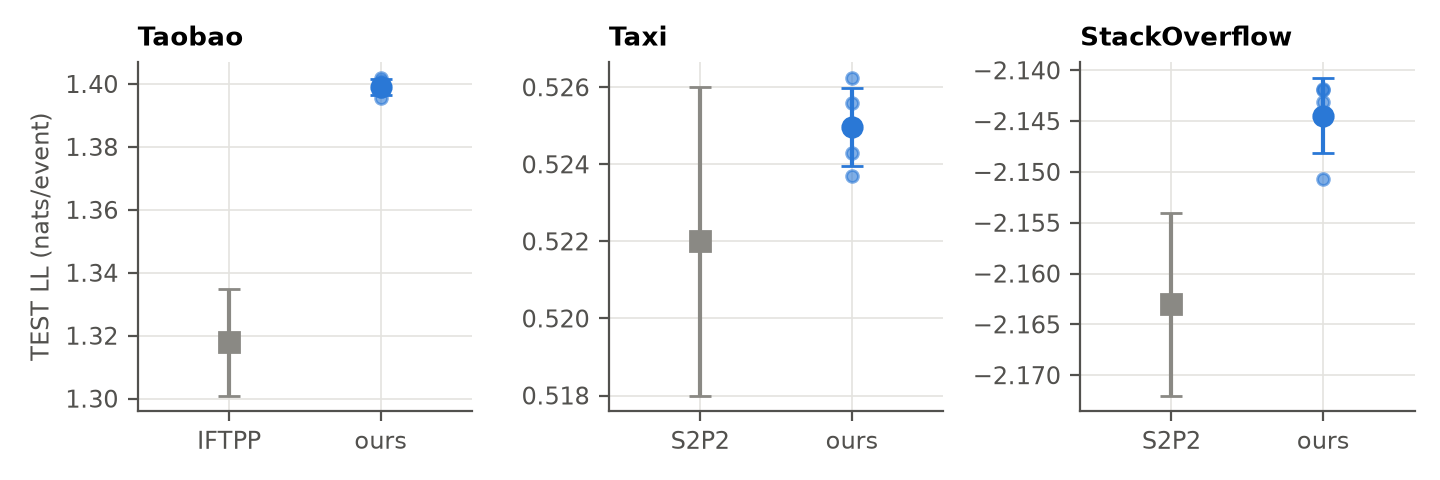
\includegraphics[width=\linewidth]{b1_results.png}
\caption{TEST log-likelihood: best published model (mean $\pm$ sd over its five seeds) and ours (each seed, mean $\pm$ sd).}
\label{fig:results}
\end{figure}

\begin{figure}[t]
\centering
\begin{minipage}{0.49\linewidth}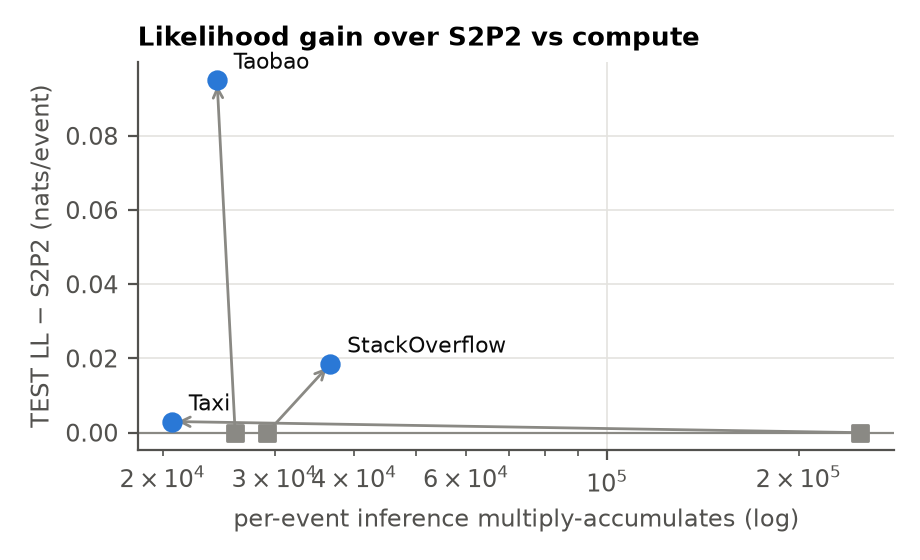
\includegraphics[width=\linewidth]{b1_compute.png}\caption{Gain over S2P2 against per-event compute.}\label{fig:compute}\end{minipage}\hfill
\begin{minipage}{0.49\linewidth}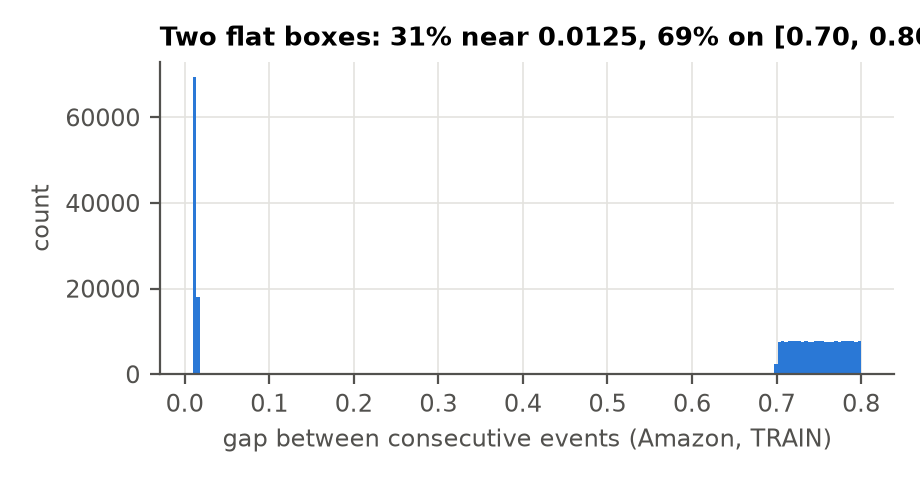
\includegraphics[width=\linewidth]{b1_amazon_gaps.png}\caption{Amazon training gaps form two flat boxes.}\label{fig:amazon}\end{minipage}
\end{figure}

\begin{figure}[t]
\centering
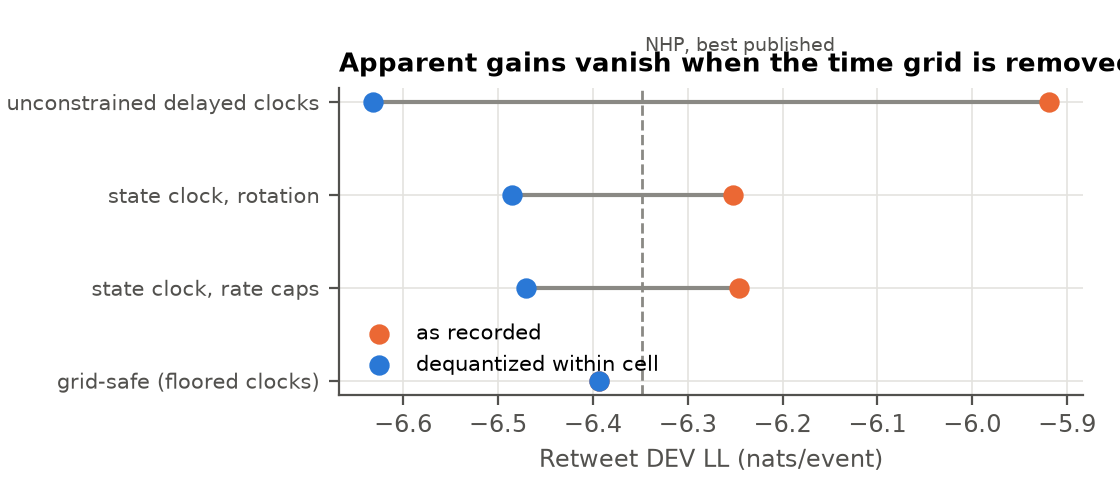
\includegraphics[width=0.8\linewidth]{b1_audit.png}
\caption{The recording-resolution pitfall on Retweet: apparent gains vanish under dequantization; the grid-safe model is unaffected.}
\label{fig:audit}
\end{figure}

\section{Ablations}
From the development log (DEV, single seeds unless stated): always-firing to defective delayed clocks, Amazon $-0.229\to0.705$; log-normal tiling to logistic windows, $0.724\to0.768$; quantile to clustered window initialization, best seeds $0.797$ with remaining seed variance; state clock on StackOverflow, $-2.173\to-2.143$. Wider encoders overfit these small datasets (Amazon $0.661$ at width 64 vs.\ $0.720$ at 32), and long training with decoupled or asymmetric weight decay did not recover past early selection.

\section{Discussion and limitations}
The race-of-clocks head gives exact likelihoods with time-dependent marks at small size; on Taxi a model with 20.5K parameters exceeds a 252K-parameter state-space model. Amazon's optimization has distinct basins; we use restart selection on DEV and report its threefold training cost. Retweet's grid-safe models do not yet exceed NHP. The encoder recurrence is sequential; its linear part admits a parallel scan. The audit applies to any continuous-time model evaluated on gridded timestamps.

\paragraph{Reproducibility.} Drivers, numerical contracts, the audit, the estimator-parity check, compute accounting and all result files are in the accompanying repository (\texttt{experiments/tpp/}, \texttt{experiments/results/tpp/}).

\bibliographystyle{plainnat}
\bibliography{refs}
\end{document}
